\section{离线性能与能耗建模}
\sectionen{Offline Performance and Energy Modeling}

\subsection{Motivation}
同一请求可以在 M 实例上完成，也可以经 P 处理输入后交给 D 继续生成。分离能够减轻阶段间干扰，却增加 KV 交接与资源配置成本。因此，规划器需要统一的性能与能耗接口，比较完整候选方案，而不只比较某次 prefill 的速度。
\EN{A request can complete on a mixed instance or pass from a prefill instance to a decode instance. Separation can reduce interference but introduces KV handoff and configuration costs. Planning therefore needs a common performance and energy interface for comparing complete candidates, rather than isolated prefill speed.}

\subsection{Challenge}
成本随输入长度、并发 batch、上下文长度、频率和实例布局变化。M 中的 prefill 还会影响正在解码的请求。另一方面，每条分离请求的 KV 交接与一次资源配置切换是不同事件，不能合并计费；超出模型覆盖范围的预测也不能作为可行性的证据。
\EN{Costs vary with prompt length, concurrent batch, context, frequency, and layout. Prefill on a mixed instance also affects ongoing decode work. Per-request KV handoff and resource reconfiguration are distinct events and need separate accounting. Predictions outside the model's coverage cannot establish that a candidate is feasible.}

\subsection{Insight}
把成本拆成可复用的 prefill、decode、混合干扰、KV 交接与状态切换组成项。离线模块提供服务时间、功率及适用范围；planning 结合负载分布、实例数量和排队估计，判断哪些配置满足 SLO，以及分离是否值得。
\EN{Decompose cost into reusable prefill, decode, mixed-interference, handoff, and state-transition components. Offline modeling provides service times, power, and validity ranges. Planning combines these with demand, replica counts, and queueing estimates to check SLOs and decide whether separation is worthwhile.}

\subsection{Approach}
\textbf{从条件到模型。}固定模型、硬件及并行布局，在代表性长度、batch、上下文和频率下采样。采集稳定窗口内的 token 时序、功率和实际频率，再拟合或插值。参数冻结后，使用新采集的独立样本检查误差与覆盖范围；未通过检查的区域不能被当作可靠预测。
\EN{Fix the model, hardware, and parallel layout, then sample representative lengths, batches, contexts, and frequencies. Record token timing, power, and actual clocks during steady windows. Fit or interpolate, freeze the parameters, and check fresh independent samples. An unqualified region cannot be treated as reliable coverage.}

图~\ref{fig:model} 用同一合成模型贯穿条件选择、查询与输出。该测试模型直接构造系数；图中的采样与验证链条是方法示意，表格与曲线则是可复算的模型响应，不是 GPU 实测或拟合验收结果。
\EN{Figure~\ref{fig:model} uses one synthetic model throughout. Its coefficients are constructed directly. Sampling and validation depict the intended method; tables and curves are reproducible model responses, not GPU measurements or evidence of a completed fitting audit.}

\begin{figure*}[t]
  \centering
  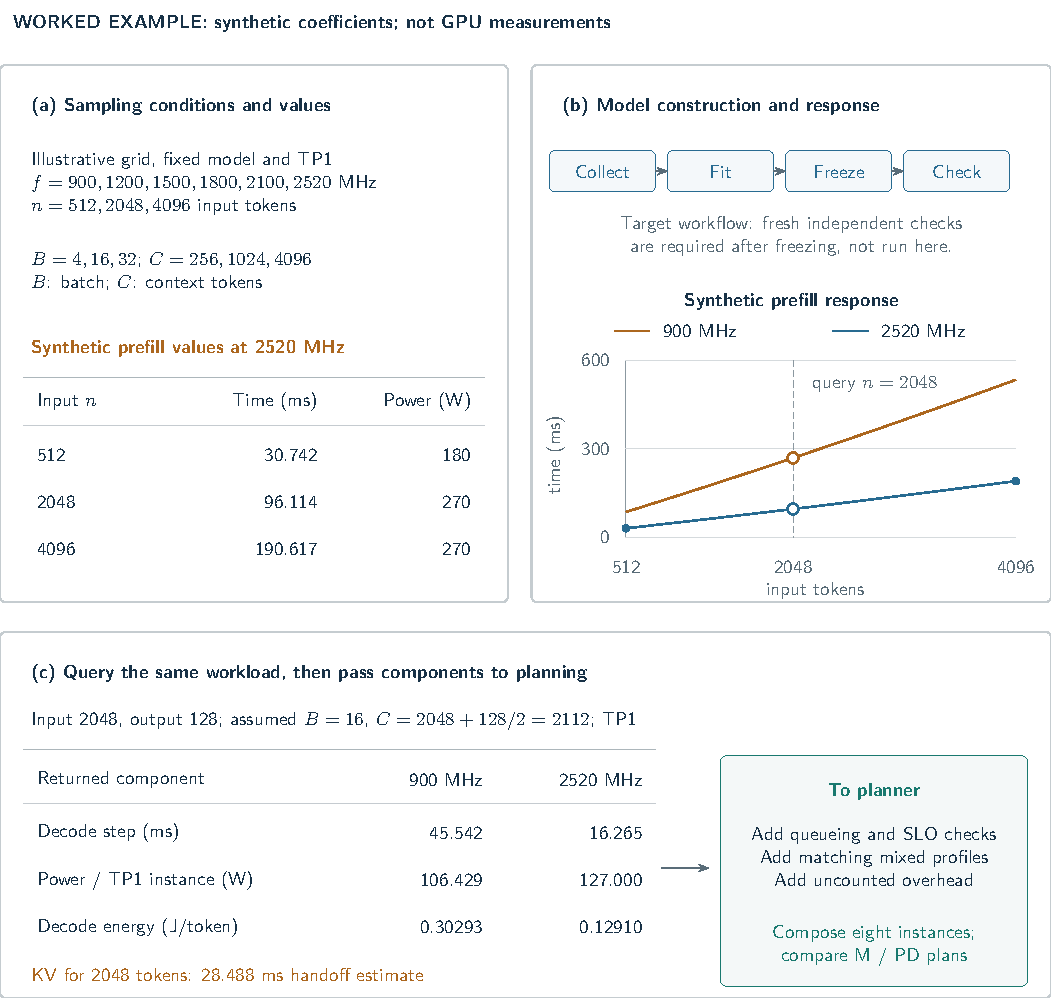
\includegraphics[width=\textwidth]{figures/02-model.pdf}
  \caption{离线模型的完整查询实例。(a) 代表性采样条件及合成响应；(b) 目标建模流程与两频率响应曲线；(c) 同一请求形状的数值查询进入规划器。全部数值来自共享六频率合成模型，功率按单个 TP1 实例计；独立硬件验证并未在此图中执行。\\\textit{A worked offline-model query: (a) illustrative sampling conditions and synthetic responses; (b) the modeling workflow and two frequency-response curves; (c) numerical queries passed to planning. All values use the shared six-frequency synthetic model and per-TP1-instance power. This figure does not perform independent hardware validation.}}
  \label{fig:model}
\end{figure*}

\textbf{从模型到查询。}实例请求包含 2048 个输入 token、128 个输出 token。假设候选稳定 batch 为 16，以 $2048+128/2=2112$ 作为代表性上下文。这两个量是候选负载假设，不能误称为实际观测。2520~MHz 下，模型返回 decode step 为 16.265~ms、功率为 127~W，因此
\begin{equation}
  \begin{aligned}
  E_{\mathrm{token}}&=\frac{\text{step time}\times\text{power}}{\text{batch}}\\
  &=\frac{0.01626496\times127}{16}\approx0.1291\;\mathrm{J/token}.
  \end{aligned}
\end{equation}
\EN{The example has 2048 input and 128 output tokens. Assume a candidate steady batch of 16 and a representative context of 2112. These are workload assumptions, not observations. At 2520~MHz, the model returns a 16.265~ms decode step and 127~W, giving approximately 0.1291~J per generated token across the batch.}

\textbf{保持接口边界。}decode step 不是请求的完整延迟。KV 交接查询返回 28.488~ms，也不是用户可见 TTFT；后者截止于客户端收到 P 产生的首 token。规划器仍须计算排队、续接间隙与完整配置的能量，并计入同一 GPU 范围内的运行和停驻功耗。交接及切换只加入基础模型尚未计入的增量。
\EN{A decode step is not end-to-end request latency. The 28.488~ms handoff estimate is not user-visible TTFT, which ends when the client receives P's first token. Planning must still evaluate queueing, continuation gaps, and configuration energy, including operating and standby power over the same GPU scope. Add only overhead not already included in the base model.}

\implnote{当前实现已有基础性能与功率模型、覆盖检查、KV 交接时间及部分切换成本，M 功率采用时间占比近似。统一、独立验证的增量交接能耗仍属于目标设计；本图的合成模型没有为这些扩展提供实测资格。}{Current code includes performance and power models, coverage checks, handoff timing, and partial switching costs; mixed power uses a time-share approximation. Uniformly validated incremental handoff energy remains a design target. The synthetic example does not qualify these extensions with hardware evidence.}
